\documentclass[tikz,border=3pt]{standalone}
\usepackage{newtxtext}
\usetikzlibrary{arrows.meta,calc,fit,positioning}

\begin{document}
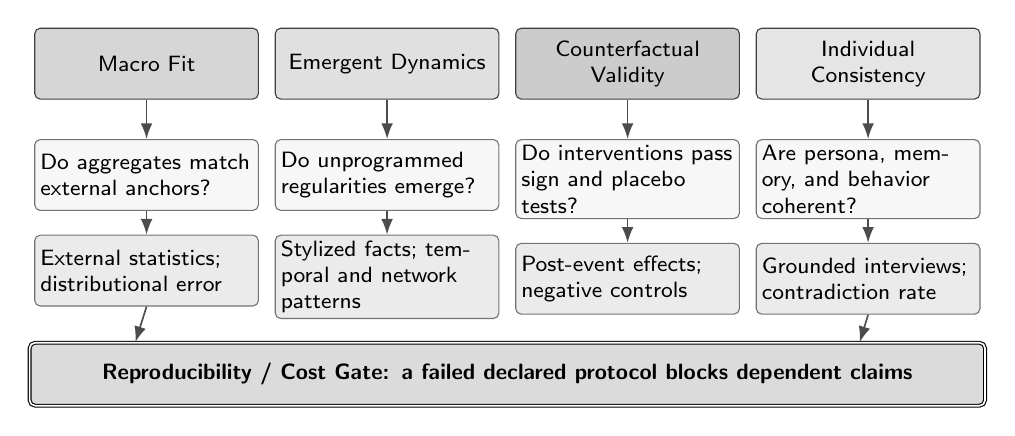
\begin{tikzpicture}[
  font=\sffamily\footnotesize,
  layer/.style={draw=black!75, rounded corners=2pt, minimum height=9mm,
    text width=27mm, align=center, inner sep=2pt},
  question/.style={draw=black!55, rounded corners=2pt, minimum height=9mm,
    text width=27mm, align=left, inner sep=2pt, fill=black!3},
  evidence/.style={draw=black!55, rounded corners=2pt, minimum height=9mm,
    text width=27mm, align=left, inner sep=2pt, fill=black!8},
  arrow/.style={-{Latex[length=2mm]}, semithick, draw=black!70}
]
  \node[layer, fill=black!16] (macro) {Macro Fit};
  \node[layer, fill=black!12, right=2mm of macro] (emergent) {Emergent Dynamics};
  \node[layer, fill=black!20, right=2mm of emergent] (causal) {Counterfactual Validity};
  \node[layer, fill=black!10, right=2mm of causal] (individual) {Individual Consistency};

  \node[question, below=5mm of macro] (qmacro) {Do aggregates match external anchors?};
  \node[question, below=5mm of emergent] (qemergent) {Do unprogrammed regularities emerge?};
  \node[question, below=5mm of causal] (qcausal) {Do interventions pass sign and placebo tests?};
  \node[question, below=5mm of individual] (qindividual) {Are persona, memory, and behavior coherent?};

  \node[evidence, below=3mm of qmacro] (emacro) {External statistics; distributional error};
  \node[evidence, below=3mm of qemergent] (eemergent) {Stylized facts; temporal and network patterns};
  \node[evidence, below=3mm of qcausal] (ecausal) {Post-event effects; negative controls};
  \node[evidence, below=3mm of qindividual] (eindividual) {Grounded interviews; contradiction rate};

  \draw[arrow] (macro) -- (qmacro);
  \draw[arrow] (emergent) -- (qemergent);
  \draw[arrow] (causal) -- (qcausal);
  \draw[arrow] (individual) -- (qindividual);
  \draw[arrow] (qmacro) -- (emacro);
  \draw[arrow] (qemergent) -- (eemergent);
  \draw[arrow] (qcausal) -- (ecausal);
  \draw[arrow] (qindividual) -- (eindividual);

  \node[draw=black, double, rounded corners=2pt, below=4mm of $(emacro.south)!0.5!(eindividual.south)$,
    text width=119mm, align=center, minimum height=8mm, fill=black!14,
    font=\sffamily\bfseries\footnotesize] (gate)
    {Reproducibility / Cost Gate: a failed declared protocol blocks dependent claims};
  \draw[arrow] (emacro.south) -- ($(gate.north west)+(13.5mm,0)$);
  \draw[arrow] (eindividual.south) -- ($(gate.north west)+(105.5mm,0)$);
\end{tikzpicture}
\end{document}
